\documentclass[12pt]{article}
\usepackage[a4paper]{geometry}
\usepackage[myheadings]{fullpage}
\usepackage{fancyhdr}
\usepackage{lastpage}
\usepackage{graphicx, wrapfig, subcaption, setspace, booktabs}
\usepackage[T1]{fontenc}
\usepackage[font=small, labelfont=bf]{caption}
\usepackage{fourier}
\usepackage[protrusion=true, expansion=true]{microtype}
\usepackage[spanish]{babel}
\usepackage{sectsty}
\usepackage{url, lipsum}
\usepackage{hyperref}
\usepackage{fancyhdr,lipsum}


\hypersetup{
    colorlinks=true, %set true if you want colored links
    linktoc=all,     %set to all if you want both sections and subsections linked
    linkcolor=blue,  %choose some color if you want links to stand out
}
\urlstyle{same}


\newcommand{\HRule}[1]{\rule{\linewidth}{#1}}
\onehalfspacing

\setcounter{secnumdepth}{2}
\setcounter{tocdepth}{5}

%-------------------------------------------------------------------------------
% HEADER & FOOTER
%-------------------------------------------------------------------------------
\pagestyle{fancy}
\fancyhf{}
\setlength\headheight{15pt}
\fancyhead[L]{SSII}
\fancyhead[R]{\uppercase{Operaciones con sistemas de virtualización}}
\fancyfoot[R]{Page \thepage\ of \pageref{LastPage}}

%-------------------------------------------------------------------------------
% TITLE PAGE
%-------------------------------------------------------------------------------

\begin{document}

\title{ \normalsize \textsc{SISTEMAS INFORMÁTICOS\\
I.E.S FRANCISCO DE LOS RÍOS}
		\\ [2.0cm]
		\HRule{0.5pt} \\
		\LARGE \textbf{\uppercase{Operaciones con sistemas de virtualización}}
		\HRule{2pt} \\ [0.5cm]
		\normalsize  \vspace*{10\baselineskip}}

\author{
        Trabajo realizado por: \\
		Antonio Muñoz Cubero
	    \normalsize  \vspace*{4\baselineskip}
		}
\date{\textbf{14 de Enero de 2021}}
\newpage
\maketitle
\newpage

%-------------------------------------------------------------------------------
% Table of Content
\tableofcontents
\newpage
%-------------------------------------------------------------------------------

%-------------------------------------------------------------------------------
% Section title formatting
\sectionfont{\scshape}
%-------------------------------------------------------------------------------






%-------------------------------------------------------------------------------
% BODY
%-------------------------------------------------------------------------------


    \section*{Introducción}
      En esta práctica de \textbf{Sistemas Informáticos} del \textit{I.E.S Francisco de los Ríos} realizaré una serie de operaciones en 
      el sistema de virtualización \href{https://www.virtualbox.org/}{\textbf{Virtual Box}}, siendo estas operaciones documentadas de 
      manera escrita y acompañadas de capturas de pantalla que ilustran el desarrollo de las mismas.
      \\\\
      El documento ha sido formateado en \LaTeX , considerando que es una opción muy válida para la realización de documentos técnicos, 
      prácticas o divulgación científica.

    \section{Instantáneas}
      En este punto de la práctica se nos pide: \textit{Realizar una instantánea de un sistema invitado, y realizar una operación con carácter 
      destructivo para acto seguido volver al estado guardado en la instantánea.}
      \\\\
      Bien, para esta primera operación, antes que nada, debemos haber descargado y configurado nuestro software de virtualización asi como 
      también deberíamos haber instalado y configurado un sistema operativo. En este caso el sistema operativo en el que desarrollaremos las 
      operaciones será \textbf{"Windows XP"} ya que el profesor, nos ha proporcionado una imagen del mismo.

      Después de la puesta a punto de nuestro sistema de virtualización, lo primero es arrancar la máquina y proceder a realizar una instantánea.
      Para ello, pulsamos sobre el desplegable que hay en nuestro sistema operativo que hemos montado y seleccionamos la opción: \textbf{Instantáneas}.
      \begin{figure}[h]
        \centering
        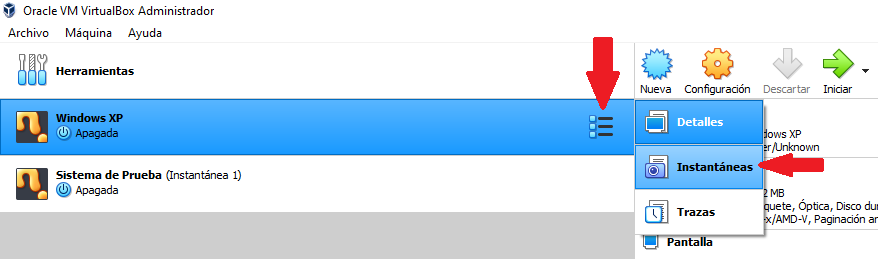
\includegraphics[scale = 0.5]{img/instantanea1.png}
        \caption{Seleccionamos la pestaña Instantánea.}
        \label{Instantanea1}
      \end{figure}

      \newpage

      Seguidamente seleccionamos la opción: \textbf{"Tomar"} o podemos usar el atajo \texttt{CTRL + SHIFT + T}, tal como se muestra en la captura.
      \begin{figure}[h]
        \centering
        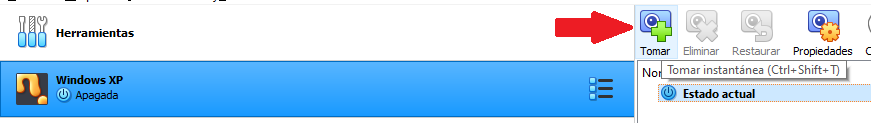
\includegraphics[scale = 0.5]{img/instantanea2.png}
        \caption{Realizamos la instantánea.}
        \label{Instantanea2}
      \end{figure}
      \\
      Nos aparecerá una ventana donde incluiremos el nombre de la Instantánea y una descripción para tenerlo todo ordenado y bien localizable.
      \begin{figure}[h]
        \centering
        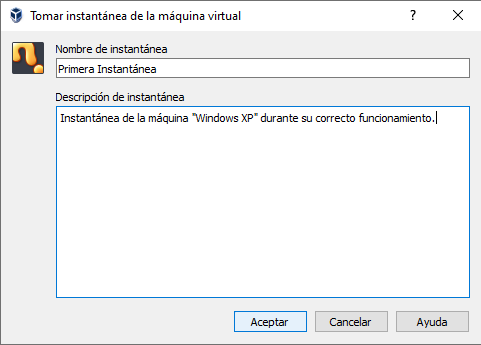
\includegraphics[scale = 1]{img/instantanea3.png}
        \caption{Descripción de la instantánea.}
      \end{figure}
      \label{Instantanea3}
      \\
      Ahora, después de realizar todos los pasos, deberíamos ver algo así en nuestro sistema de virtualización.
      \begin{figure}[h]
        \centering
        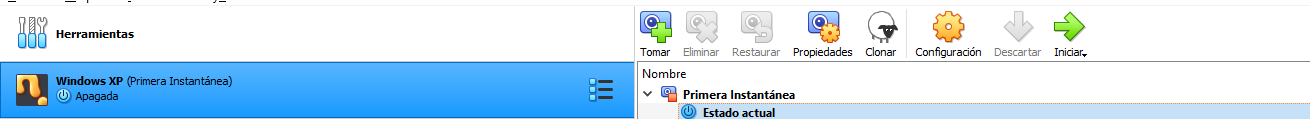
\includegraphics[scale = 0.5]{img/instantanea4.png}
        \caption{Resultado final de la captura de instantáneas.}
        \label{Instantanea4}
      \end{figure}

      \newpage

      El siguiente paso es realizar una operación que inhabilite a la máquina virtual, para seguidamente restaurarla usando la 
      instantánea que acabamos de crear.
      \\
      Para inhabilitar la máquina virtual, ejecutaría el comando \texttt{erase c:/WINDOWS} pero no tengo permiso de administrador,
      además la contraseña no la se, al ser una iso preinstalada. Pero eso debería bastar para inhabilitarlo.
      \begin{figure}[h]
        \centering
        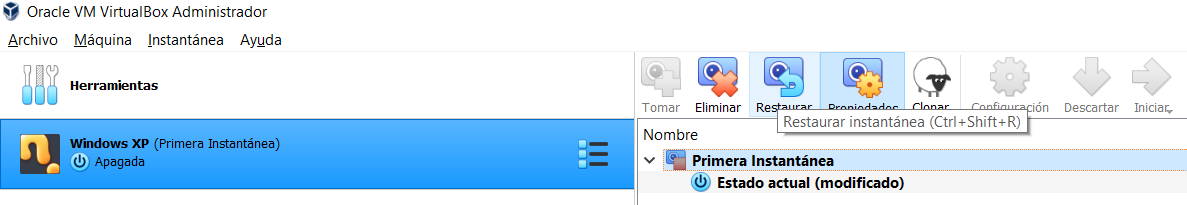
\includegraphics[scale = 0.6]{img/instantanea5.png}
        \caption{Restauramos la Instantánea.}
        \label{Instantanea5}
      \end{figure}
      \\
      Una vez nuestra máquina no esté en posición de ser ejecutada correctamente, nos vamos al menú de Instantáneas de la máquina invitada 
      que deseemos restaurar y pulsamos en la Instantánea creada y pulsamos restaurar, tal y como se muestra en la imagen anterior. Así pues, 
      nos quedaraía la máquina en el estado en el que creamos la captura. 
      \begin{figure}[h]
        \centering
        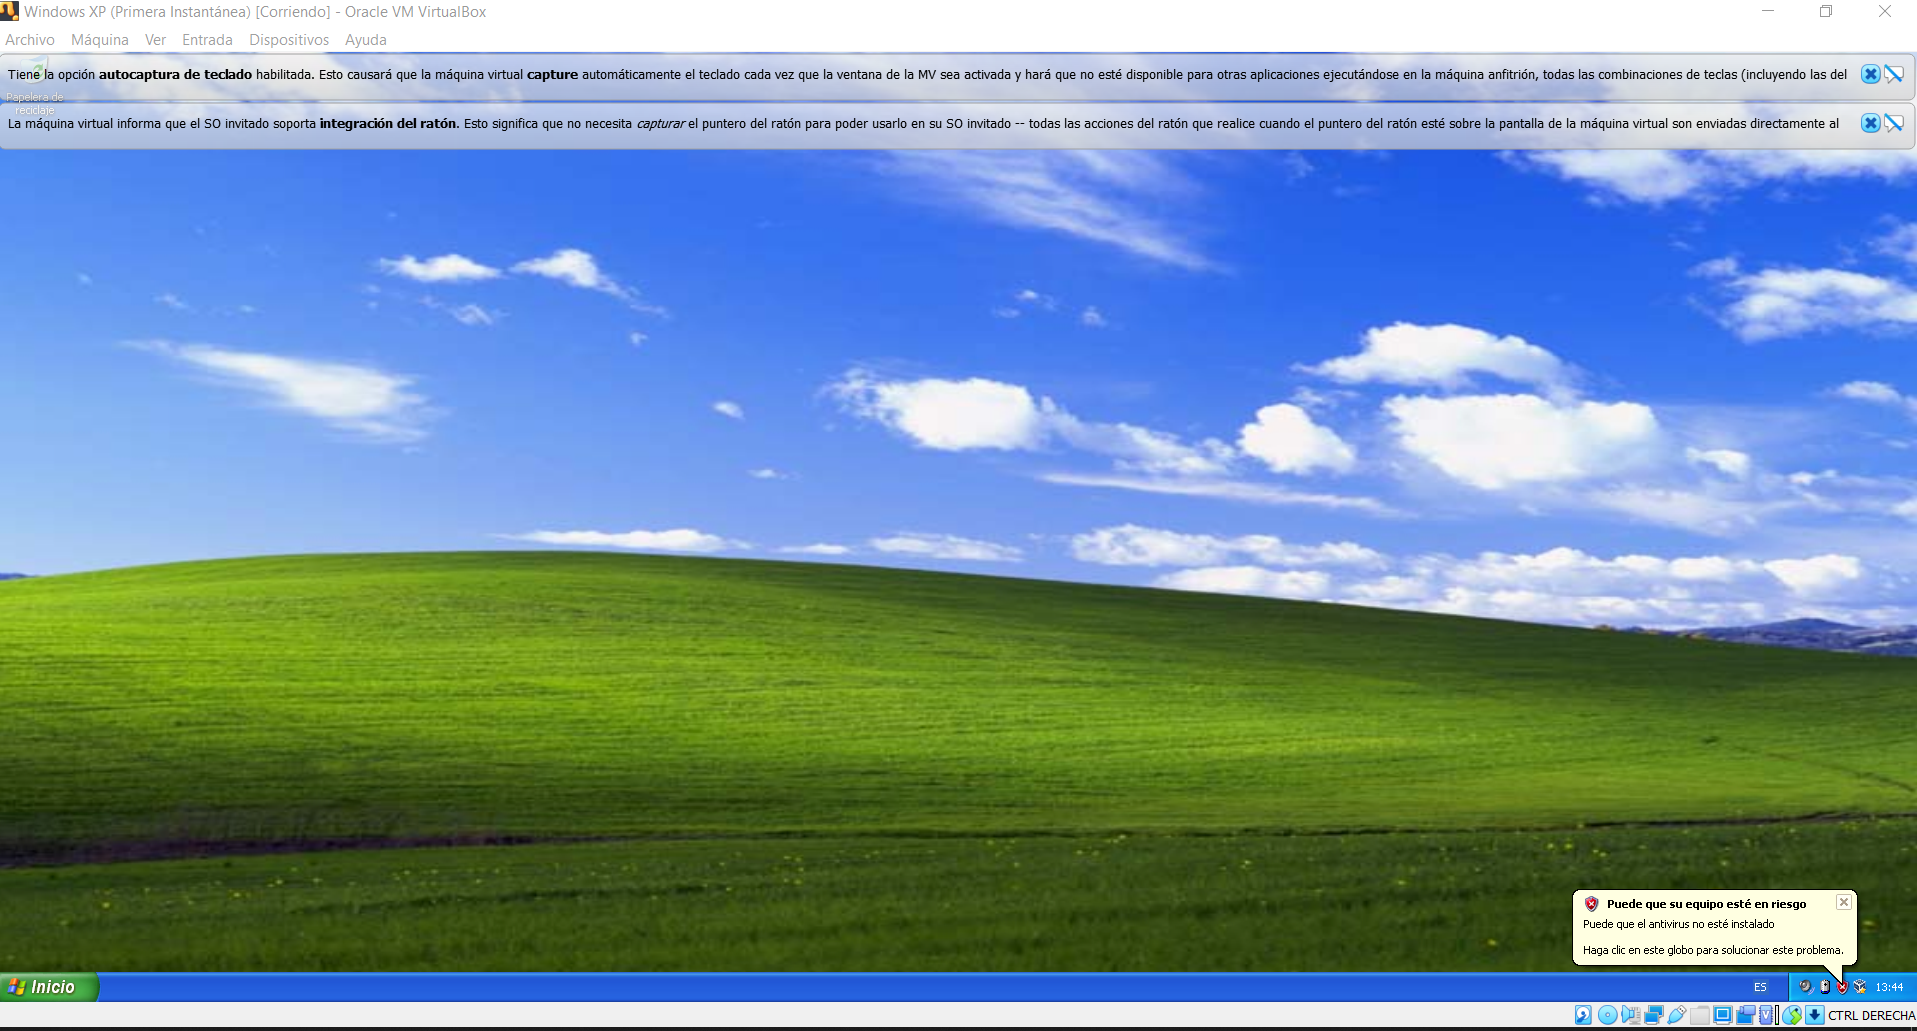
\includegraphics[scale = 0.35]{img/instantanea6.png}
        \caption{Imagen restaurada.}
        \label{Instantanea6}
      \end{figure}
      
      \newpage
    
    \section{Clonado}
      En este apartado \textit{realizaremos un clonado de un sistema invitado en un disco independiente comprobando que 
      podemos ejecutar los dos sistemas simultaneamente.}
      \\
      Para realizar el clonado de una máquina nos iremos al mismo menú de \textbf{la figura }\ref{Instantanea1}.
      y pulsamos en el boton de \textbf{Clonar}, nos aparecerá una ventana con las opciones que tenemos que seleccionar 
      para la realización del clonado.
      \begin{figure}[h]
        \centering
        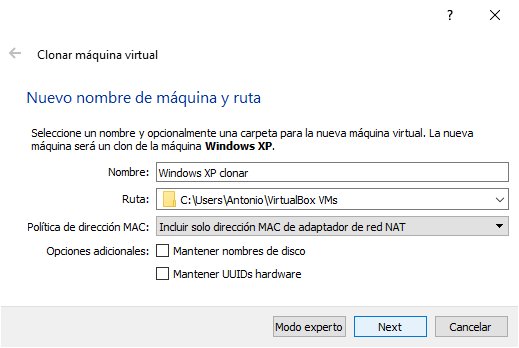
\includegraphics[scale = 0.75]{img/clonar1.png}
        \caption{Opciones para el clonado.}
        \label{Clonado1}
      \end{figure}
      Debemos nombrar a la maquina clonada, la ruta donde se guardaría la máquina, la política de la dirección MAC, y unas 
      operaciones adicionales y pulsamos \textit{"next"}.
      \begin{figure}[h]
        \centering
        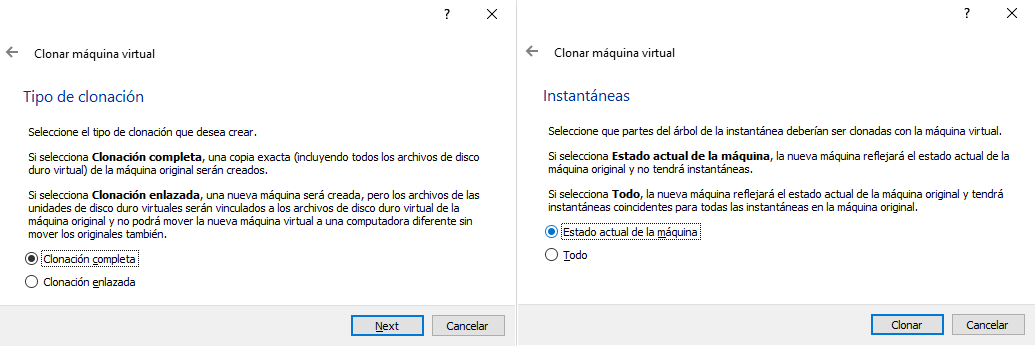
\includegraphics[scale = 0.5]{img/clonar2.png}
        \caption{Diferentes ventanas para el clonado.}
        \label{Clonado2}
      \end{figure}
      Seguidamente nos aparecerá un par de ventanas donde tenemos que elegir si clonar la máquina enlazadamente o una clonación 
      completa e incluso el monmento de clonación de la máquina, si el actual o algún otro.

      \newpage

      En el siguiente paso de este apartado debemos ejecutar a la vez las dos máquinas que hemos creado, \textit{Windows XP y Windows XP clonar}.
      \begin{figure}[h]
        \centering
        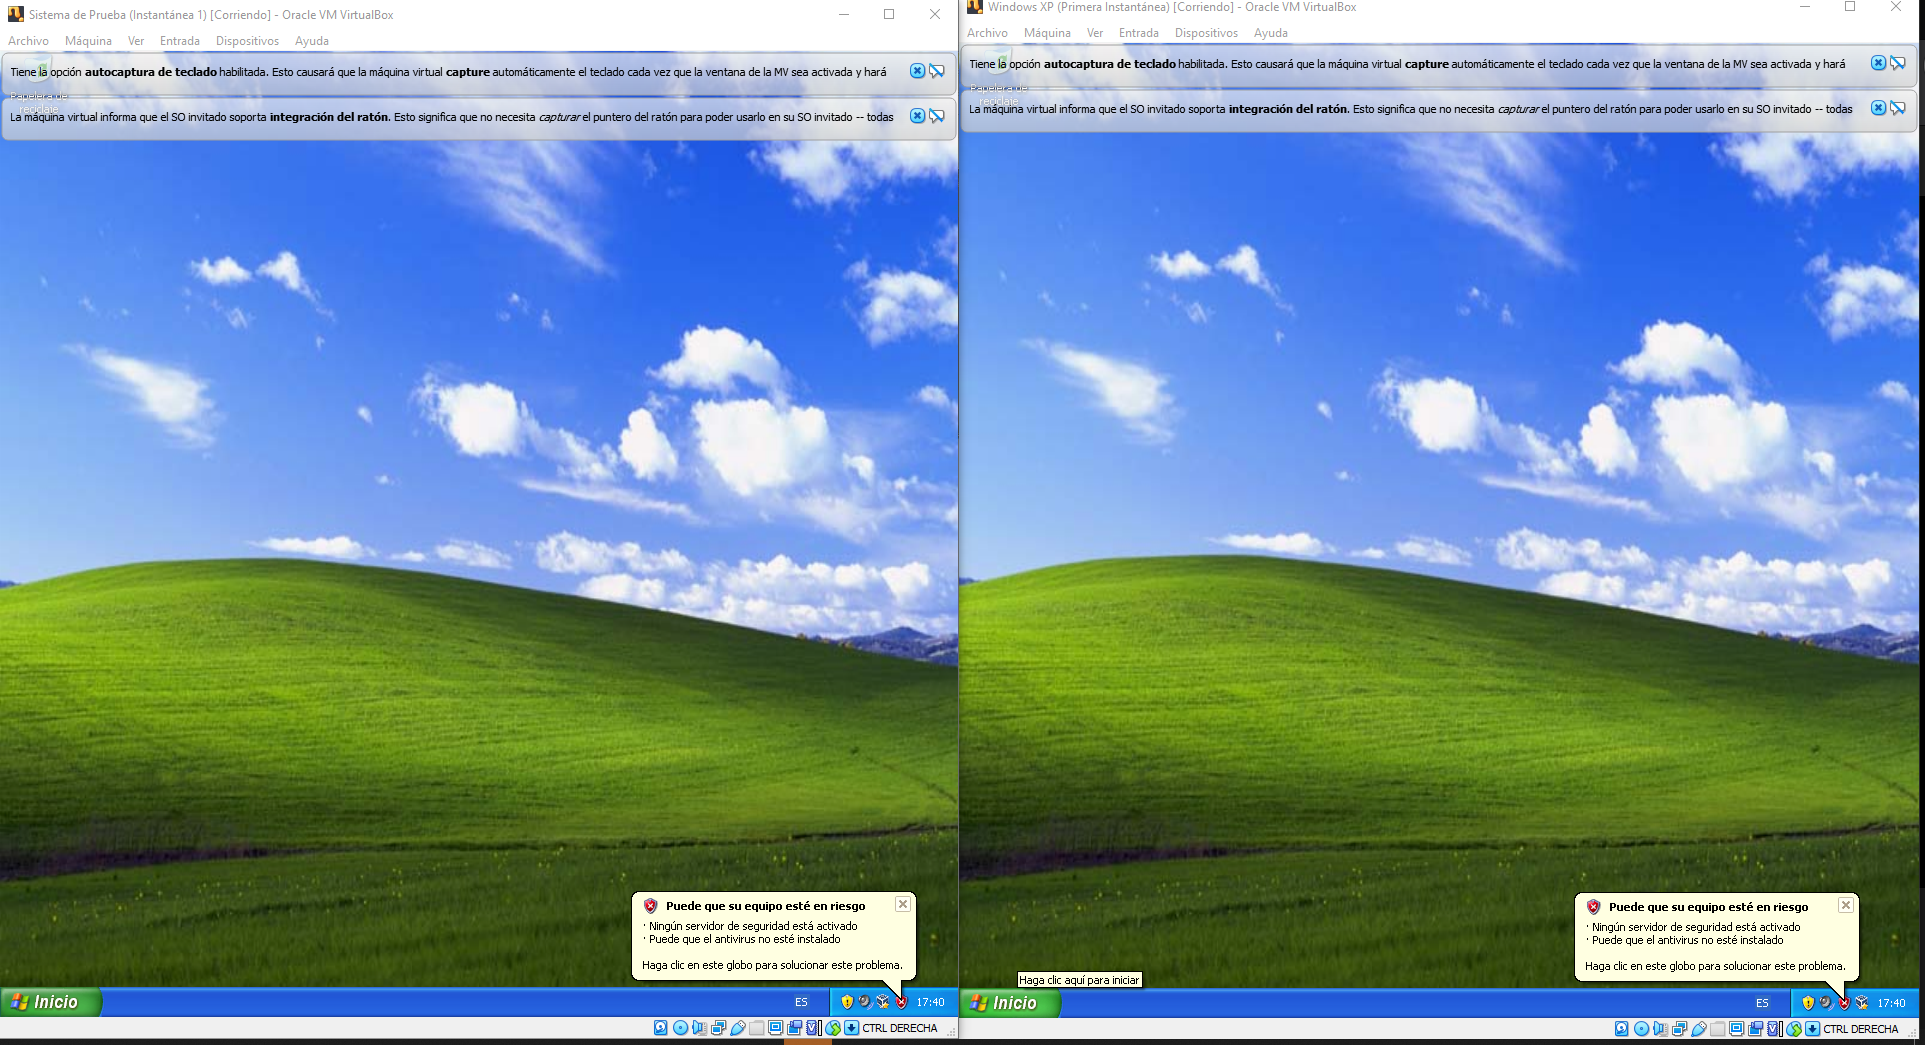
\includegraphics[scale = 0.3]{img/clonar3.png}
        \caption{Dos máquinas corriendo a la vez.}
        \label{Clonado3}
      \end{figure}
      \\
      Vemos que efectivamente, el posible correr las dos máquinas virtuales a la vez.

      \newpage

    \section{Configuración de red modo NAT}
      \textit{En este apartado comprobaremos el direccionamiento y la conectividad desde el sistema invitado al anfitrión y viceversa.}
      \\\\
      En primer lugar debemos comprobar que el protocolo de la tarjeta de red de nuestra máquina es el adecuado, en el caso de 
      este apartado el modo \textbf{NAT}. Lo haremos pulsando en el botón de red y comprobamos que esté puesto el modo \textbf{NAT}.
      \\
      \begin{figure}[h]
        \centering
        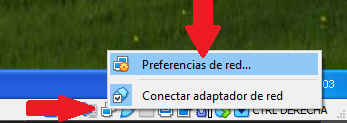
\includegraphics{img/clonar4.png}
        \caption{Botón de red.}
        \label{Nat}
      \end{figure}
      \\
      \begin{figure}[h]
        \centering
        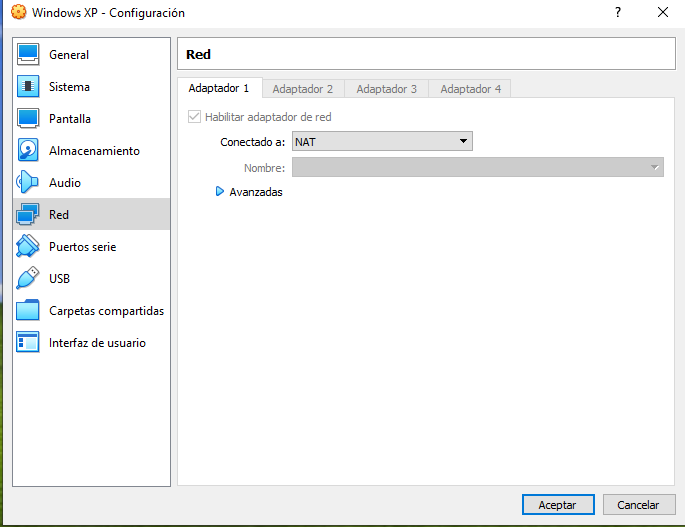
\includegraphics[scale = 0.5]{img/clonar5.png}
        \caption{Opción de red.}
        \label{Nat2}
      \end{figure}

      \newpage

      La dirección de nuestra máquina invitada es: \texttt{10.0.2.15} y la dirección de nuestra máquina anfitrión es: \texttt{192.168.1.35}, 
      para conprobar el direccionamiento debejemos ejecutar el comando \texttt{ping} desde la máquina que deseemos junto con la ruta de la 
      máquina a la que queremos comprobar el direccionamiento.
      \\
      Primeramente desde la máquina anfitrión comprobamos el direccionamiento hacia la máquina invitada, haciendo uso de lo comentado anteriormente.
      El resultado sería el siguiente:
      \\
      \begin{figure}[h]
        \centering
        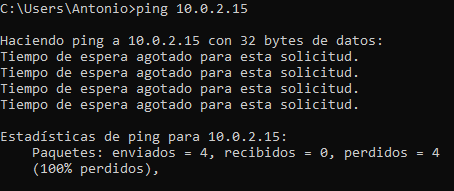
\includegraphics{img/nat1.png}
        \caption{Resultado del ping a máquina invitada.}
        \label{Nat3}
      \end{figure}
      \\
      Podemos comprobar que el direccionamiento de red desde la máquina anfitrión a la máquina invitada no está funcionando.
      \\\\
      Seguidamente, comprobamos la operación viceversa.
      \begin{figure}[h]
        \centering
        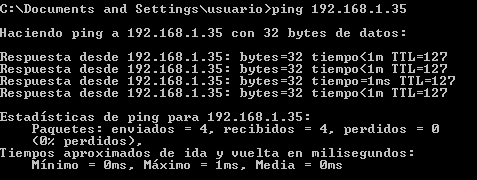
\includegraphics{img/nat2.png}
        \caption{Resultado del ping a máquina anfitrión.}
        \label{Nat4}
      \end{figure}
      \\
      En esto caso podemos comprobar que funciona perfectamente.

      \newpage

    \section{Configuración de red modo BRIDGE(puente)}
      \textit{En este apartado debemos comprobar el direccionamiento y la conectividad desde el sistema invitado al anfitrión y viceversa.}
      \\\\
      Con el modo \textbf{BRIDGE} o puente, nuestra máquina invitada será visible en todo el espectro de red del dispositivo anfitrión 
      y también para dispositivos externos.
      \\
      Para configurar el BRIDGE, tenemos que irnos al mismo apartado en el que tuvimos que entrar en el apartado anterior, las \textbf{
      preferencias de red.} \ref{Nat} Una vez dentro, elegimos la opción, \textit{conectado a: "Adaptador puente"}. Tal como se muestra 
      en la imagen.
      \begin{figure}[h]
        \centering
        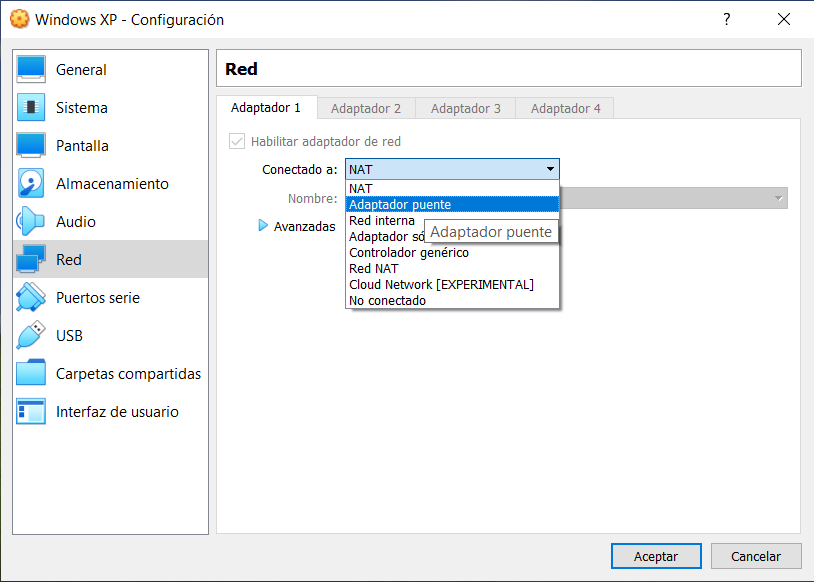
\includegraphics[scale = 0.75]{img/bridge1.png}
        \caption{Conectado a Adaptador puente.}
        \label{Bridge1}
      \end{figure}
      Muy importante, no debemos olvider seleccionar el Adaptador de red que esté usando nuestra máquina anfitrión, en mi caso, usé el 
      adaptador wireless de INTEL, ya que estoy usando una red WIFI.

      \newpage

      Ahora comprobaremos la conexión entre ambas máquinas, para comprobara que la funcionalidad del adaptador BRIDGE es totalmente funcional 
      y no tendremos ningún problema de conexión.
      \\\\
      Nuestro router le ha asignado a la máquina anfitrión la ip \texttt{192.168.1.35} y a la máquina invitada \texttt{192.168.1.84}. Teniendo 
      esto en cuenta, este es el resultado de realizar las comprobaciones de conexión.
      \begin{figure}[h]
        \centering
        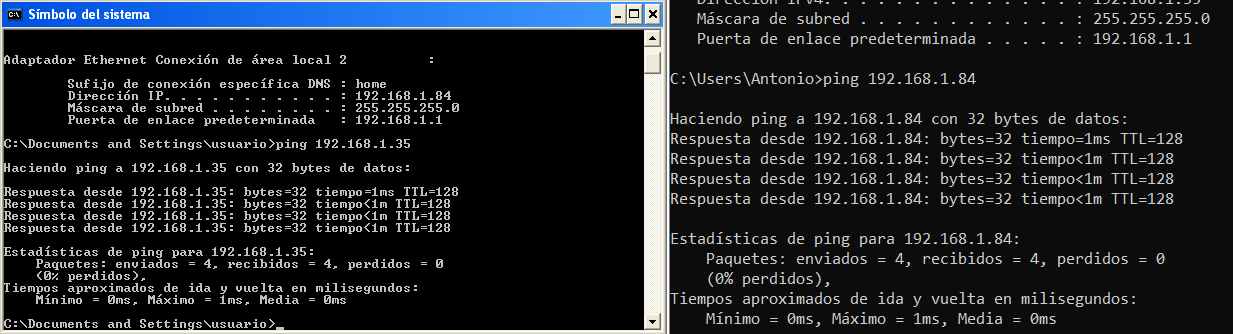
\includegraphics[scale = 0.6]{img/bridge2.png}
        \caption{comprobaciones de conexiones.}
        \label{Bridge2}
      \end{figure}
      \\
      Como podemos comprobar, no tenemos ningún probrema para conectarnos entre ambas máquinas desde la terminal que deseemos, por lo tanto, esta 
      es una de las opciones más interesante y a tener en cuenta.

      \newpage

    \section{Configuración de red modo RED NAT}
      \textit{En este último apartado configuraremos nuestra máquina virtual con la opción de red en domo \textbf{RED NAT} y seguidamente comprobaremos el 
      direccionamiento de ambas máquinas para comprobar su conectividad.}
      \\
      Para la configuracon de la máquina virtual en modo \textit{RED NAT}. Primero debemos crear una configuración de red NAT, con ello, nuestra 
      máquina virtual tendrá la posibilidad de utilizar de manera efectiva esta opción. Para ello, desde la ventana principal de VirtualBox, seleccionamos 
      la ruta \texttt{Archivo -> Preferencias} o podemos usar el atajo \texttt{Crtl + G} seleccionamos el apartado de \texttt{Red} 
      \begin{figure}[h]
        \centering
        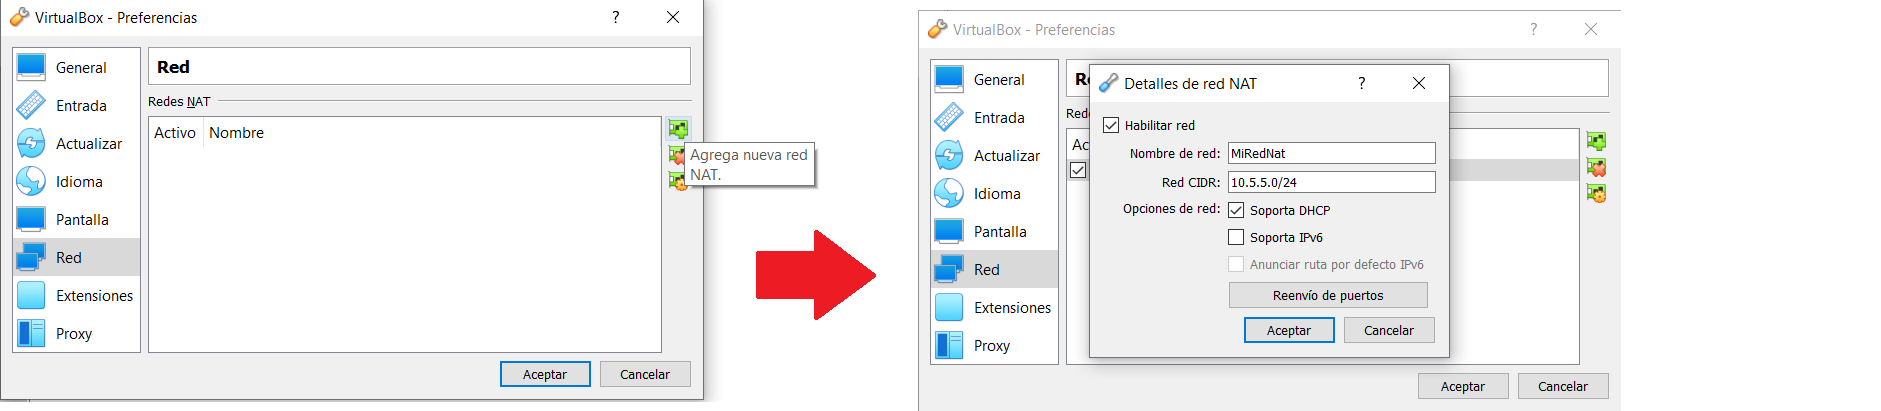
\includegraphics[scale = 0.45]{img/RedNAT1.png}
        \caption{Configuracion de RED NAT.}
        \label{RedNAT1}
      \end{figure}
      \\
      Una vez en la pestaña, pulsamos en agregar una nueva red y configuramos la misma, las opciones que vemos en la imagen pueden ser una opción válida para 
      diferenciar la red del invitado.
      \\
      Seguidamente nos vamos al mismo apartado que en los anteriores apartados, \textbf{Preferencias de red.} \ref{Nat} Y seleccionamos la opción \textbf{RED NAT} 
      y seleccionamos la Configuración que hemos creado, en este caso \textit{MiRedNAt} y pulsamos \textit{Aceptar}.
      \begin{figure}[h]
        \centering
        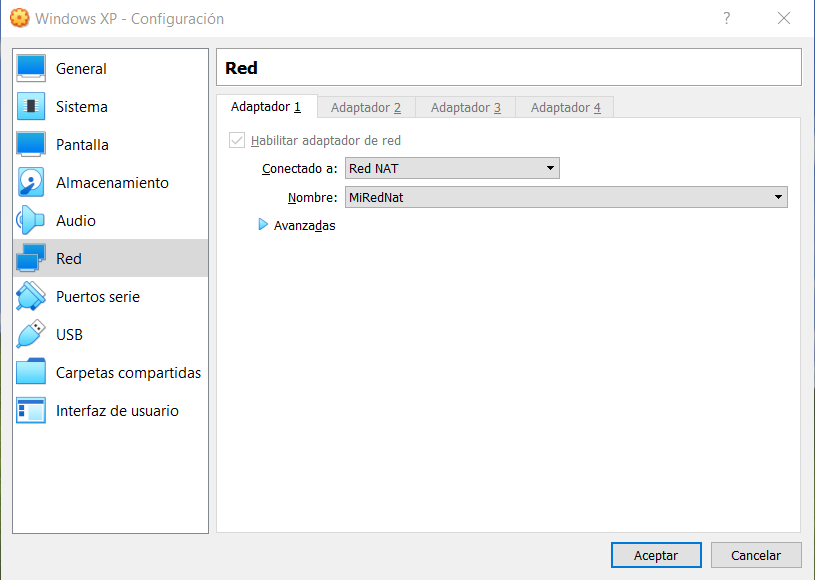
\includegraphics[scale = 0.4]{img/RedNAT2.png}
        \caption{Preferencias de RED.}
        \label{RedNAT2}
      \end{figure}

      \newpage

      En primer lugar comprobaremos la contectividad entre máquina anfitrión y maquina invitada, para ello, como siempre abrimos la consola de comandos en la máquina 
      invitada para comprobar que las configuraciones de red se han realizado correctamente, mendiente el comando \texttt{ipconfig} y después de comprobar que efectivamente
      nos han proporcionado una IP acorde a lo configurado, procedemos a hacer \texttt{ping} a la máquina anfitrión.
      \begin{figure}[h]
        \centering
        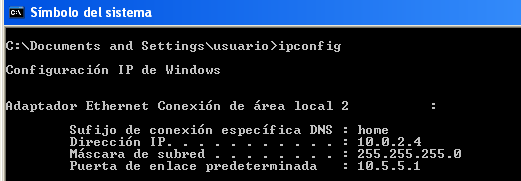
\includegraphics[scale = 1]{img/RedNAT3.png}
        \caption{direccionamiento IP erróneo.}
        \label{RedNAT3}
      \end{figure}
      \\
      Sin embargo, observamos que el direccionamiento IP no es el correcto, ya que nuestra Configuración era \texttt{10.5.5.0} y nos da una distinta, se deberá a un fallo de 
      software o algo que se escapa de mi conocimiento, por tanto, procederemos a configurar la dirección IP de forma manual.
      \\
      Nos dirigimos a la ruta \texttt{Panel de control, Conexiones de Red e Internet, Conexiones de Red} y una vez en ese directorio, pulsamos botón derecho sobre \textit{Conexion
      de área local 2} y nos vamos a \textit{Propiedades}.
      \begin{figure}[h]
        \centering
        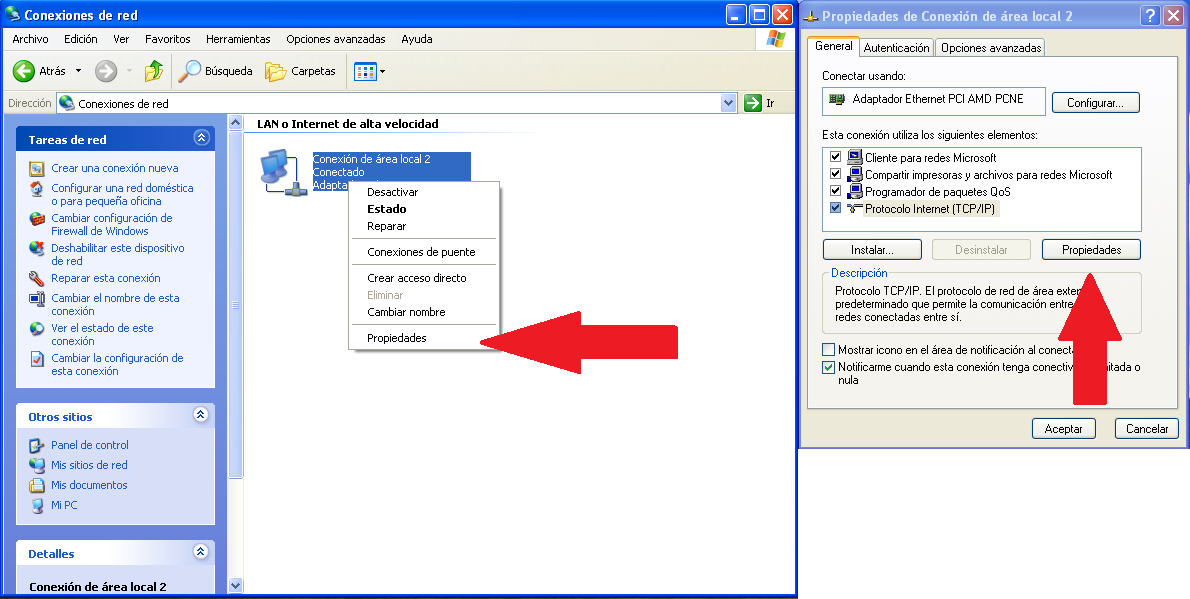
\includegraphics[scale = 0.5]{img/RedNAT4.png}
        \caption{Configuración manual de la IP.}
        \label{RedNAT4}
      \end{figure}
      
      \newpage

      Seleccionamos el protocolo \textit{TCP/IP} y añadimos la siguiente configuración y pulsamos aceptar.
      \begin{figure}[h]
        \centering
        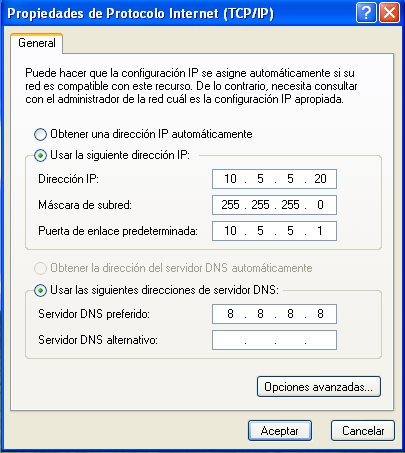
\includegraphics[scale = 0.9]{img/RedNAT5.png}
        \caption{Configuracion del TCP/IP.}
        \label{RedNAT5}
      \end{figure}
      \\
      Comprobamos que tenemos ahora bien la configuración NAT usando el comando \texttt{ipconfig} en la 
      consola de comando, como hicimos anteriormente.
      \begin{figure}[h]
        \centering
        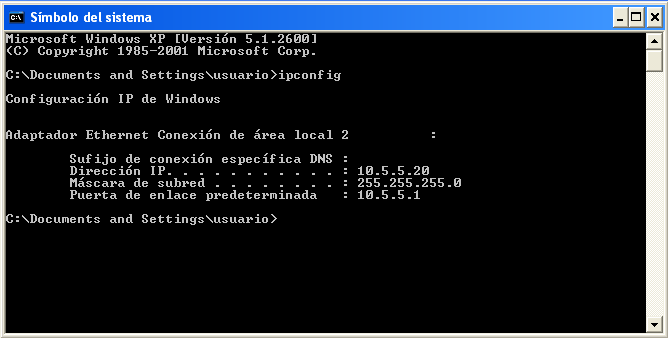
\includegraphics[scale = 0.8]{img/RedNAT6.png}
        \caption{Comprobación de la IP.}
        \label{RedNAT6}
      \end{figure}
      \\
      Efectivamente, ahora si tenemos bien configurada nuestra dirección IP, por tanto, podemos proceder a comprobar 
      la conectividad entre las diferentes máquinas.

      \newpage

      Primero hacemos ping desde la máquina invitada a la anfitrión y seguidamente desde la máquina anfitrión a la máquina 
      invitada.
      \begin{figure}[h]
        \centering
        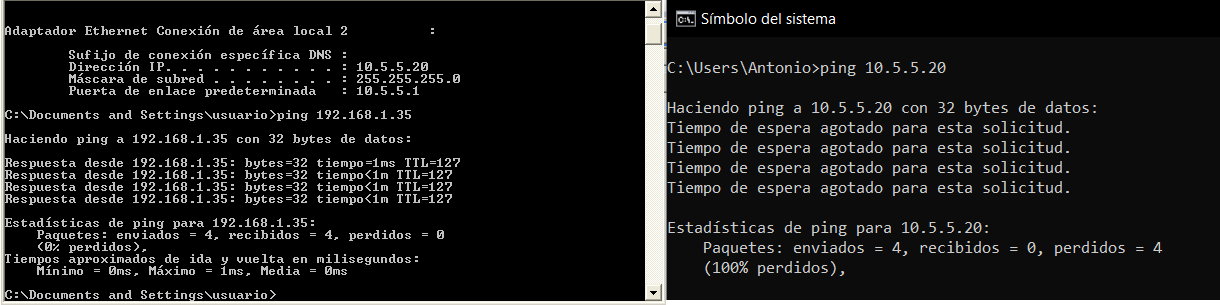
\includegraphics[scale = 0.6]{img/RedNAT7.png}
        \caption{Comprobación de conexiones.}
        \label{RedNAT7}
      \end{figure}
      \\
      Comprobamos que hay conexión de la máquina invitada a la anfitrión, pero no viceversa.
      \\\\
      Ahora comprobamos, haciendo un clonado de la máquina invitada, si hay conexión entre las dos máquinas invitadas, teniendo 
      en cuenta que en una de ellas debemos cambiar la dirección IP, en mi caso, una máquina tendrá la dirección \texttt{10.5.5.20} 
      y otra la dirección \texttt{10.5.5.30}.
      \begin{figure}[h]
        \centering
        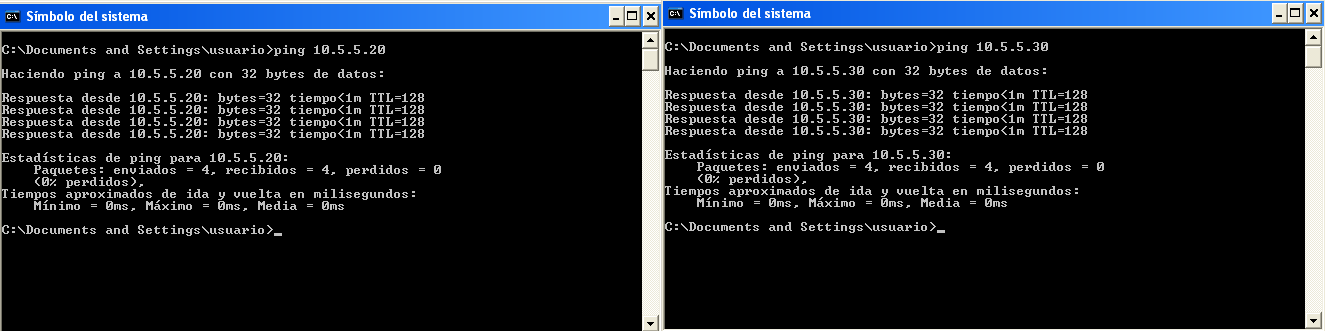
\includegraphics[scale = 0.55]{img/RedNAT8.png}
        \caption{Comprobación de conexiones entre dos invitados.}
        \label{RedNAT8}
      \end{figure}
      \\
      Podemos comprobar que se pueden comunicar entre ellas sin ningún tipo de problema.

      \newpage

    \section{IMÁGENES}
      \listoffigures
\end{document}